\documentclass[11pt,a4paper]{ctexart}
\usepackage{fontspec}
\defaultfontfeatures{Mapping=tex-text}
\usepackage{xunicode}
\usepackage{xltxtra}
\usepackage{amsmath}
\usepackage{amsfonts}
\usepackage{amssymb}
\usepackage{graphicx}
\usepackage{amsthm}
\usepackage{array}
\usepackage{tcolorbox}
\usepackage{float}   %{H}
\usepackage{booktabs}  %\toprule[1.5pt]
\usepackage[titletoc]{appendix}
%===================%插入代码需要的控制
\usepackage{listings}
\usepackage{xcolor}
\setmonofont{Consolas}%字体
\lstset{
	keywordstyle= \color{ blue!70},
	commentstyle= \color{red!50!green!50!blue!50}, 
	frame=shadowbox, % 阴影效果
	rulesepcolor= \color{ red!20!green!20!blue!20} ,
	escapeinside=``,% 英文分号中可写入中文
	basicstyle=\ttfamily 
} 
%===================%
\usepackage[left=2cm,right=2cm,top=2cm,bottom=2cm]{geometry}
\newtheorem*{solution}{解}

\title{多元统计分析(4)}
\author{钟瑜 \quad 222018314210044}
\date{\today}
\begin{document}
	\maketitle
	\pagestyle{plain}%设置页码
\begin{figure}[H]
	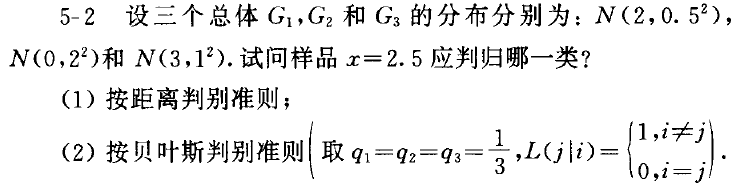
\includegraphics[width=0.7\textwidth]{screenshot001}
\end{figure}
\begin{solution}
\begin{enumerate}
	\item[(1)] 
	\begin{equation}
		\begin{aligned}
			d(x,G_1)&=\frac{(x-\mu_1)^2}{\sigma_1^2}=1\\
			d(x,G_2)&=\frac{(x-\mu_2)^2}{\sigma_2^2}=1.5625\\
			d(x,G_3)&=\frac{(x-\mu_3)^2}{\sigma_3^2}=0.25\\
		\end{aligned}
	\end{equation}
由于$ d(x,G_3) $最小,故应判归第三类.
	\item[(2)] 由于
\begin{lstlisting}[language=r]
> dnorm(2.5,2,0.5)
[1] 0.4839414
> dnorm(2.5,0,2)
[1] 0.09132454
> dnorm(2.5,3,1)
[1] 0.3520653
\end{lstlisting}

而$ q_1=q_2=q_3=1 $,$$ q_2f_2=0.09132454<q_3f_3=0.3520653<q_1f_1=0.4839414$$

由推论
\begin{figure}[H]
	\centering
	
\includegraphics[width=0.7\linewidth]{screenshot007}
\end{figure}
故判归第一类.
\end{enumerate}
\end{solution}
%=======================================================================================
\begin{figure}[H]
	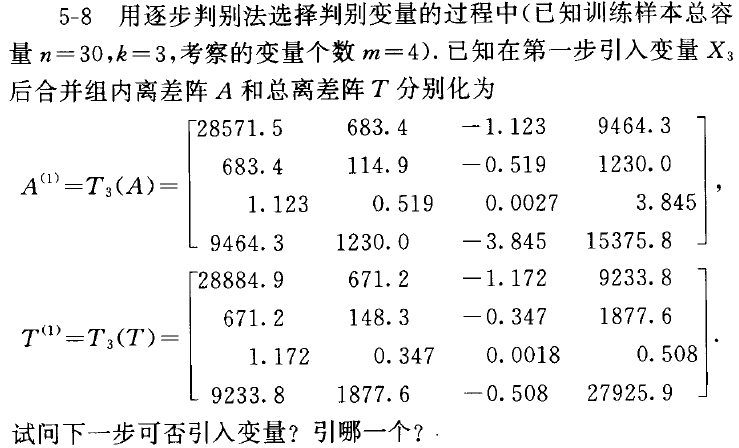
\includegraphics[width=0.7\textwidth]{screenshot002}
\end{figure}
\begin{solution}
\end{solution}
\begin{lstlisting}[language=r]
> #n=30,k=3
> A<-matrix(c(28571.5,683.4,-1.123,9464.3,
+             683.4,1149,-0.519,1230.0,
+             1.123,0.519,0.0027,3.845,
+             9464.3,1230.0,-3.845,15375.8),byrow = TRUE,ncol=4)
> T<-matrix(c(28884.9,671.2,-1-172,9233.8,
+             671.2,148.3,-0.347,1877.6,
+             1.172,0.347,0.0018,0.508,
+             9233.8,1877.6,-0.508,27925.9),byrow=TRUE,ncol=4)
> lambda<-det(A)/det(T)
> lambda
[1] 10.68135
\end{lstlisting}

%=======================================================================================
\begin{figure}[H]
	
\includegraphics[width=0.7\textwidth]{screenshot003}
\end{figure}
\begin{figure}[H]
	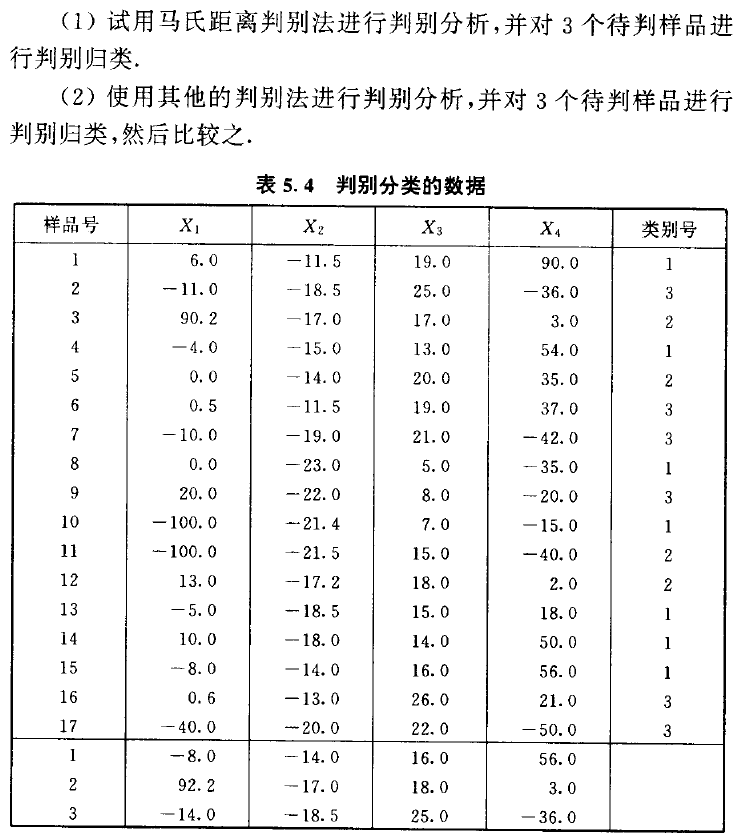
\includegraphics[width=0.7\linewidth]{screenshot004}
\end{figure}
\begin{solution}
\end{solution}
(1)
\begin{lstlisting}[language=r]
> data<-read.csv("E:/4.多元统计分析/zuoye/4/10.csv")
> data$type<-as.factor(data$type)
> str(data)
'data.frame':	20 obs. of  5 variables:
$ x1  : num  6 -11 90.2 -4 0 0.5 -10 0 20 -100 ...
$ x2  : num  -11.5 -18.5 -17 -15 -14 -11.5 -19 -23 -22 -21.4 ...
$ x3  : int  19 25 17 13 20 19 21 5 8 7 ...
$ x4  : int  90 -36 3 54 35 37 -42 -35 -20 -15 ...
$ type: Factor w/ 3 levels "1","2","3": 1 3 2 1 2 3 3 1 3 1 ...

DDAM<-function (TrnX, TrnG, TstX = NULL, var.equal = FALSE){ #多元距离判别函数
	if ( is.factor(TrnG) == FALSE){
		mx<-nrow(TrnX); mg<-nrow(TrnG)
		TrnX<-rbind(TrnX, TrnG)
		TrnG<-factor(rep(1:2, c(mx, mg)))
	}
	if (is.null(TstX) == TRUE) TstX<-TrnX
	if (is.vector(TstX) == TRUE)  TstX<-t(as.matrix(TstX))
	else if (is.matrix(TstX) != TRUE)
	TstX<-as.matrix(TstX)
	if (is.matrix(TrnX) != TRUE) TrnX<-as.matrix(TrnX)
	nx<-nrow(TstX)
	blong<-matrix(rep(0, nx), nrow=1, dimnames=list("blong", 1:nx))
	g<-length(levels(TrnG))
	mu<-matrix(0, nrow=g, ncol=ncol(TrnX))
	for (i in 1:g)
	mu[i,]<-colMeans(TrnX[TrnG==i,]) 
	D<-matrix(0, nrow=g, ncol=nx)
	if (var.equal == TRUE  || var.equal == T){
		for (i in 1:g)
		D[i,]<- mahalanobis(TstX, mu[i,], var(TrnX))
	}
	else{
		for (i in 1:g)
		D[i,]<- mahalanobis(TstX, mu[i,], var(TrnX[TrnG==i,]))
	}
	for (j in 1:nx){
		dmin<-Inf
		for (i in 1:g)
		if (D[i,j]<dmin){
			dmin<-D[i,j]; blong[j]<-i
		}
	}
	blong
}

> G<-gl(3,20)
> X<-data[,-5]
> DDAM(X,G)
Error in TrnX[TrnG == i, ] : (下标)逻辑下标太长 
\end{lstlisting}
(2)线性判别分析:
\begin{lstlisting}[language=r]
> library(MASS)
> View(A)
> ld<-lda(data$type~data$x1+data$x2+data$x3+data$x4)
> ld
Call:
lda(data$type ~ data$x1 + data$x2 + data$x3 + data$x4)  #公式

Prior probabilities of groups: #先验概率
        1         2         3 
0.4117647 0.2352941 0.3529412 

Group means: #各组均值向量
    data$x1   data$x2  data$x3   data$x4
1 -14.42857 -17.34286 12.71429  31.14286
2   0.80000 -17.42500 17.50000   0.00000
3  -6.65000 -17.33333 20.16667 -15.00000

Coefficients of linear discriminants: #第一和第二线性判别函数系数
                 LD1          LD2
data$x1 -0.009870482 -0.022839978
data$x2 -0.542919566  0.106647088
data$x3 -0.047312575  0.024128295
data$x4  0.068388163 -0.001001915

Proportion of trace: #两个判别式对判别的贡献大小
  LD1   LD2 
0.996 0.004 
> Z<-predict(ld)
> Z
$class
[1] 1 3 3 1 2 3 3 1 1 1 2 2 1 1 1 3 3
Levels: 1 2 3

$posterior
1           2            3
1  9.890173e-01 0.010600406 3.823032e-04
2  4.776285e-05 0.097968167 9.019841e-01
3  2.740321e-03 0.446093207 5.511665e-01
4  9.820309e-01 0.017255788 7.132755e-04
5  1.432291e-01 0.560319463 2.964514e-01
6  4.703544e-03 0.318882368 6.764141e-01
7  5.519341e-05 0.106111183 8.938336e-01
8  5.551665e-01 0.385618402 5.921511e-02
9  6.323055e-01 0.327991369 3.970312e-02
10 9.859693e-01 0.013226287 8.044569e-04
11 2.413737e-01 0.463482728 2.951436e-01
12 3.019693e-02 0.528897636 4.409054e-01
13 9.102735e-01 0.083079446 6.647017e-03
14 9.988689e-01 0.001120492 1.056153e-05
15 9.410302e-01 0.054669487 4.300268e-03
16 6.245518e-04 0.190138106 8.092373e-01
17 1.271870e-04 0.117787436 8.820854e-01

$x
LD1         LD2
1   2.20029533  0.28118465
2  -2.73225351  0.19394572
3  -1.49988665 -2.18959050
4   2.02112021  0.02761879
5  -0.19184441  0.23084042
6  -1.36998966  0.45990602
7  -2.69174289  0.02728051
8   0.61694890 -1.02077375
9   0.76050442 -1.31357007
10  2.00846388  1.46207772
11 -0.02544884  1.66948725
12 -0.74500229 -0.42254338
13  1.37461015 -0.23848051
14  3.19082694 -0.58394621
15  1.51252117  0.29600685
16 -1.98199600  0.48258009
17 -2.44712675  0.63797639

> X1<-X[18:20,]
> C<-predict(ld,X1)
> C
$class
[1] 1 3 3 1 2 3 3 1 1 1 2 2 1 1 1 3 3 1 3 3
Levels: 1 2 3

$posterior
1           2            3
1  9.890173e-01 0.010600406 3.823032e-04
2  4.776285e-05 0.097968167 9.019841e-01
3  2.740321e-03 0.446093207 5.511665e-01
4  9.820309e-01 0.017255788 7.132755e-04
5  1.432291e-01 0.560319463 2.964514e-01
6  4.703544e-03 0.318882368 6.764141e-01
7  5.519341e-05 0.106111183 8.938336e-01
8  5.551665e-01 0.385618402 5.921511e-02
9  6.323055e-01 0.327991369 3.970312e-02
10 9.859693e-01 0.013226287 8.044569e-04
11 2.413737e-01 0.463482728 2.951436e-01
12 3.019693e-02 0.528897636 4.409054e-01
13 9.102735e-01 0.083079446 6.647017e-03
14 9.988689e-01 0.001120492 1.056153e-05
15 9.410302e-01 0.054669487 4.300268e-03
16 6.245518e-04 0.190138106 8.092373e-01
17 1.271870e-04 0.117787436 8.820854e-01
18 9.410302e-01 0.054669487 4.300268e-03
19 2.224781e-03 0.429111664 5.686636e-01
20 5.285885e-05 0.099358550 9.005886e-01

$x
LD1         LD2
1   2.20029533  0.28118465
2  -2.73225351  0.19394572
3  -1.49988665 -2.18959050
4   2.02112021  0.02761879
5  -0.19184441  0.23084042
6  -1.36998966  0.45990602
7  -2.69174289  0.02728051
8   0.61694890 -1.02077375
9   0.76050442 -1.31357007
10  2.00846388  1.46207772
11 -0.02544884  1.66948725
12 -0.74500229 -0.42254338
13  1.37461015 -0.23848051
14  3.19082694 -0.58394621
15  1.51252117  0.29600685
16 -1.98199600  0.48258009
17 -2.44712675  0.63797639
18  1.51252117  0.29600685
19 -1.56694019 -2.21114217
20 -2.70264207  0.26246566
\end{lstlisting}
%=======================================================================================
\begin{figure}[H]
	
\includegraphics[width=0.7\linewidth]{screenshot005}
\end{figure}
\begin{figure}[H]
	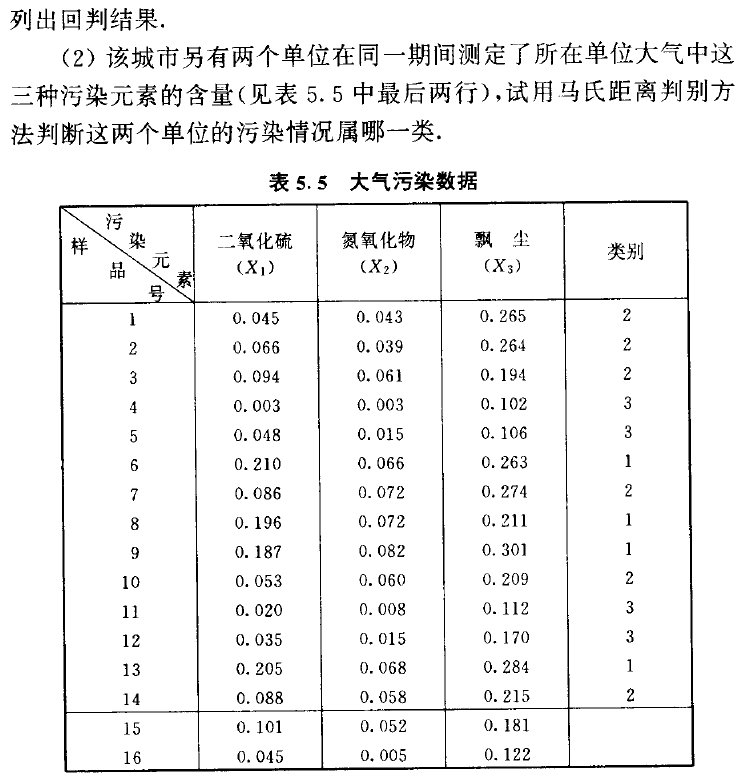
\includegraphics[width=0.7\linewidth]{screenshot006}
\end{figure}
\begin{solution}
\end{solution}
(1)若三个总体为多元正太总体,协方差阵相等,先验概率取为各类样本的比例.则
$$D^2_t(X)=d^2_t(X)+g_2(t)$$
三个总体的先验概率为
\begin{equation}
	\begin{aligned}
		q_1&=\frac{3}{7}\\
		q_2&=\frac{2}{7}\\
		q_3&=\frac{2}{7}\\
	\end{aligned}
\end{equation}
那么
\begin{equation}
	\begin{aligned}
		g_2(1)=-2ln|q_1|&=1.694596\\
		g_2(2)=-2ln|q_2|&=2.505526\\
		g_2(3)=-2ln|q_3|&=2.505526\\
	\end{aligned}
\end{equation}
\begin{lstlisting}[language=r]
> data1<-read.csv("E:/4.多元统计分析/zuoye/4/11.csv")
> data11<-data1[1:14,]
> data12<-data1[15:16,]
> d1<-data11[which(data11$type==1), ]
> d2<-data11[which(data11$type==2), ]
> d3<-data11[which(data11$type==3), ]
> s1<-cov(d1[,-4])
> s2<-cov(d2[,-4])
> s3<-cov(d3[,-4])
> mu1<-colMeans(d1[,-4])
> mu2<-colMeans(d2[,-4])
> mu3<-colMeans(d3[,-4])
> D1<-mahalanobis(d1[,-4],mu1,s1)
> D2<-mahalanobis(d2[,-4],mu2,s2)
> D3<-mahalanobis(d3[,-4],mu3,s3)
> D1;D2;D3
6    8    9   13 
2.25 2.25 2.25 2.25 
1         2         3         7        10        14 
1.9796692 2.5083563 2.1627834 4.1247155 3.3089299 0.9155458 
4    5   11   12 
2.25 2.25 2.25 2.25 

\end{lstlisting}


(2)
\begin{lstlisting}[language=r]
> D11<-mahalanobis(data12[,-4],mu1,s1)
> D22<-mahalanobis(data12[,-4],mu2,s2)
> D33<-mahalanobis(data12[,-4],mu3,s3)
> D11;D22;D33
15       16 
8368.24 33328.59 
15        16 
5.914895 38.756728 
15      16 
7020274 1944463 
\end{lstlisting}
15判为2,16判为2.
\end{document}